%%%%%%%%%%%%%%%%%%
% Based on https://github.com/jdavis/latex-homework-template
%%%%%%%%%%%%%%%%%%

\documentclass{article}

\usepackage{fancyhdr}
\usepackage{extramarks}

\usepackage{amsmath}
\usepackage{amsthm}
\usepackage{amsfonts}

\usepackage{tikz}
\usetikzlibrary{arrows.meta, positioning}

\usepackage[plain]{algorithm}
\usepackage{algpseudocode}

%\usepackage{hyperref}

%%%%%% Basic Document Settings %%%%%%%%%

\topmargin=-0.45in
\evensidemargin=0in
\oddsidemargin=0in
\textwidth=6.5in
\textheight=9.0in
\headsep=0.25in

\linespread{1.1}

%%%%%%%%%%%%%%%%%% Homework Details %%%%%%%%%%%%%%%
% Title
% Due date
% University
% Class
% Instructor
% Author
% Author ID 

\newcommand{\hmwkTitle}{Assignment\ \#1}
\newcommand{\hmwkDueDate}{Oct 29, 2022}
\newcommand{\hmwkClass}{Introduction to Artificial Intelligence (CS-487)}
\newcommand{\hmwkClassInstructor}{Professor I. Tsamardinos}
\newcommand{\hmwkUniversity}{University of Crete \\Department of Computer Science}
\newcommand{\hmwkAuthorName}{Nikolaos Kougioulis}
\newcommand{\hmwkAuthorID}{ID 1285}


\pagestyle{fancy}
\lhead{\hmwkAuthorName\ (\hmwkAuthorID)} %left head
%\chead{\hmwkClass\ \hmwkTitle} %center head
%\rhead{\date{\today}} %right head
\rhead{\hmwkClass\ \hmwkTitle} 
\lfoot{\lastxmark}
\cfoot{\thepage}

\renewcommand\headrulewidth{0.4pt}

\setlength\parindent{0pt}

\setcounter{secnumdepth}{0}
\newcounter{partCounter}
\newcounter{ExerciseCounter}
\setcounter{ExerciseCounter}{1}
\nobreak\extramarks{Exercise \arabic{ExerciseCounter}}{}\nobreak{}

%%%%%% Homework Problem Environment %%%%%%

\newenvironment{Exercise}[1][-1]{
	\ifnum#1>0
	\setcounter{ExerciseCounter}{#1}
	\fi
	\section{Exercise \arabic{ExerciseCounter}}
	\setcounter{partCounter}{1}
}{
}
% Alias for the Solution section header
\newcommand{\solution}{\textbf{\large Solution:}}

% Title Page %

\title{
	\centering
	
\includegraphics[height=1.5in]{images/background.png}
	
	 \vspace{1in}
	\textmd{\textbf{\hmwkClass\ \hmwkTitle}}\\
	
	\normalsize\vspace{0.1in}\small{Due\ on\ \hmwkDueDate}\\
	
	\vspace{0.1in}\large{\textit{\hmwkClassInstructor}} \\
	\vspace{0.5in}
	\large{\hmwkUniversity}

	\vspace{3in}
	
	\author{\textbf{\hmwkAuthorName} (\hmwkAuthorID)}
	\date{\today}
}

% Various Helper Commands %

\newcommand{\alg}[1]{\textsc{\bfseries \footnotesize #1}}
% For derivatives
\newcommand{\deriv}[1]{\frac{\mathrm{d}}{\mathrm{d}x} (#1)}
% For partial derivatives
\newcommand{\pderiv}[2]{\frac{\partial}{\partial #1} (#2)}
% Integral dx
\newcommand{\dx}{\mathrm{d}x}
\newcommand{\E}{\mathbb{E}}
\newcommand{\Var}{\mathrm{Var}}
\newcommand{\Cov}{\mathrm{Cov}}
\newcommand{\Bias}{\mathrm{Bias}}

%\def\blankpage{%
%	\clearpage%
%	\thispagestyle{empty}%
%	\addtocounter{page}{-1}%
%	\null%
%	\clearpage}

%for code listings
\usepackage{listings}
\usepackage{xcolor}

\definecolor{codegreen}{rgb}{0,0.6,0}
\definecolor{codegray}{rgb}{0.5,0.5,0.5}
\definecolor{codepurple}{rgb}{0.58,0,0.82}
\definecolor{backcolour}{rgb}{0.99,0.99,0.99}

\lstdefinestyle{mystyle}{
	backgroundcolor=\color{backcolour},   
	commentstyle=\color{codegreen},
	keywordstyle=\color{magenta},
	numberstyle=\tiny\color{codegray},
	stringstyle=\color{codepurple},
	basicstyle=\ttfamily\footnotesize,
	breakatwhitespace=false,         
	breaklines=true,                 
	captionpos=b,                    
	keepspaces=true,                 
	numbers=left,                    
	numbersep=5pt,                  
	showspaces=false,                
	showstringspaces=false,
	showtabs=false,                  
	tabsize=2
}

\lstset{style=mystyle}

\begin{document}

	\maketitle
	
	%\blankpage
	
	%\setcounter{page}{1}
	
	\begin{Exercise}[1]
		Both the performance measure and the utility function measure how well an agent does. Explain how they differ. \\
		
		\solution \\
				
		Indeed, both the performance measure and the utility function serve as a measure of how "well" an agent performs. There is however a slight difference, depending on which perspective we choose (the designer of the agent(a human) or the agent itself. \\
		
		A performance measure is in the mind of the designer of the agent, or in the mind of the users of the agent. The performance of the agent is evaluated on how preferable their sequence of actions is from the human's point of view. As such, a performance measure is objective and can include information unavailable to the agent (like in a partially observable, sequential environment). The performance measure may be explicit or implicit (the agent may perform the correct task, but have no idea why). That's why we need to assume the performance measure can be specified correctly. \\
		
		On the other hand, a utility function includes only information available to the agent itself, the states and sequence of actions. The utility function is an internalization of the performance measure itself and is ideally an estimate of the performance measure (if both the utility function and performance measure are in agreement, an agent choosing actions that maximize its utility function will be \textit{rational} according the performance measure.)
		
	\end{Exercise}
	
	\newpage
	
	\begin{Exercise}[2]
		Can such graph exist in which $A^{\star}$ extends more nodes than the Depth-First
		Search algorithm; If so, draw an example of such a graph. If not, explain why
		this is impossible. \\
		
		\solution \\
		
		We expect Depth-First Search to expand more nodes than $A^{\star}$ search with an admissible heuristic. \\ 
		
		A lucky Depth-First Search algorithm may however expand fewer nodes than $A^{\star}$, simply by expanding exactly those nodes on the optimal path to reach the goal state (if the optimal path consists of $k$ nodes, then a lucky Depth-First Search may expand exactly those $k$ nodes), without the need for backtracking (backing up to the next deepest node that has unexpanded successors). \\
		
		So in the case of a lucky Depth-First Search, $A^{\star}$ could possibly expand more nodes before finding the optimal path. Moreover, $A^{\star}$ may expand more nodes than Depth-First Search with an inadmissible heuristic. \\
		
		We illustrate an example similar to the routes of Romania problem with starting node A, final node D and heuristic function values $h(A) = 500, ~h(B) = 400, ~h(C) = 100, ~h(D) = 0, ~h(E) = 330, ~h(F) = 350$ (see \ref{fig:img1}).
		
		\begin{figure}[h]
			\centering
			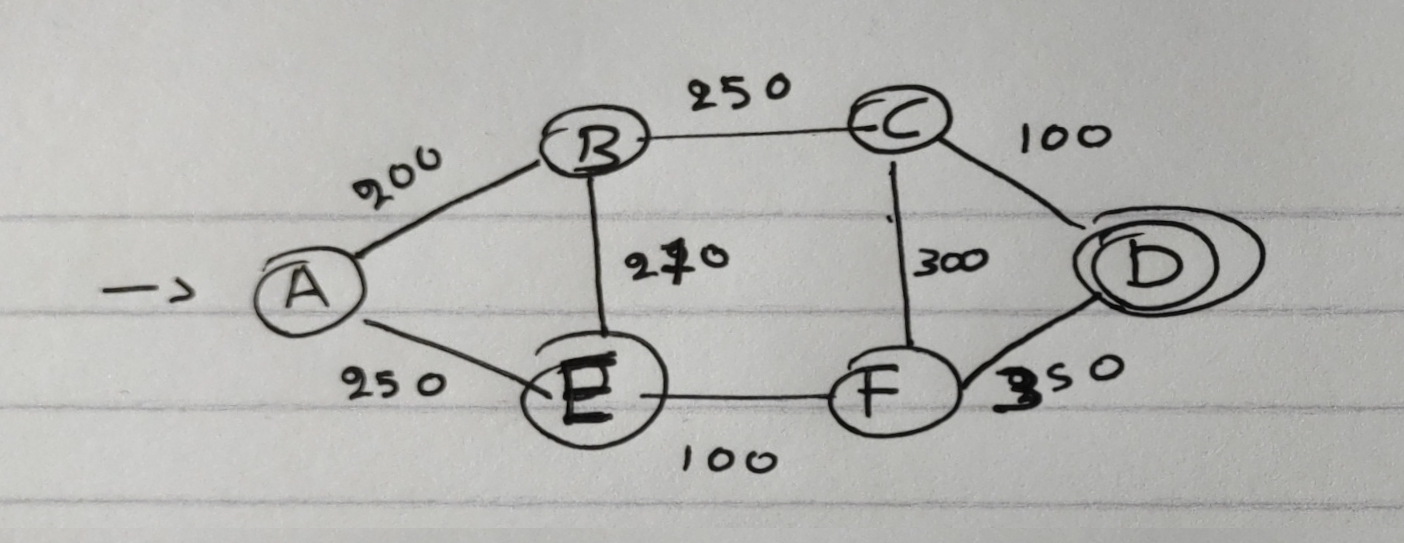
\includegraphics[width=0.45\textwidth]{images/1.jpg}
			\caption{Formulation of the state space, similar to the Romania problem, with initial state node A and final state node D.}
			\label{fig:img1}
		\end{figure}
		
		In figure \ref{fig:img2}, Depth-First Search is illustrated. Starting with the initial node, Depth-First Search always expands the deepest node on the frontier. The algorithm is being lucky since it has reached the goal state expanding those nodes on the optimal path, without the need for backtracking (after reaching the deepest level of the tree, with no more successors, returning to the next deepest node on the frontier that has unexpanded successors.). We assume that in our implementation Depth-First Search takes care checking each nodes for cycles, as to not get stuck in infinite loops due to the cyclic state space. 
		
		\begin{figure}[h]
			\centering
			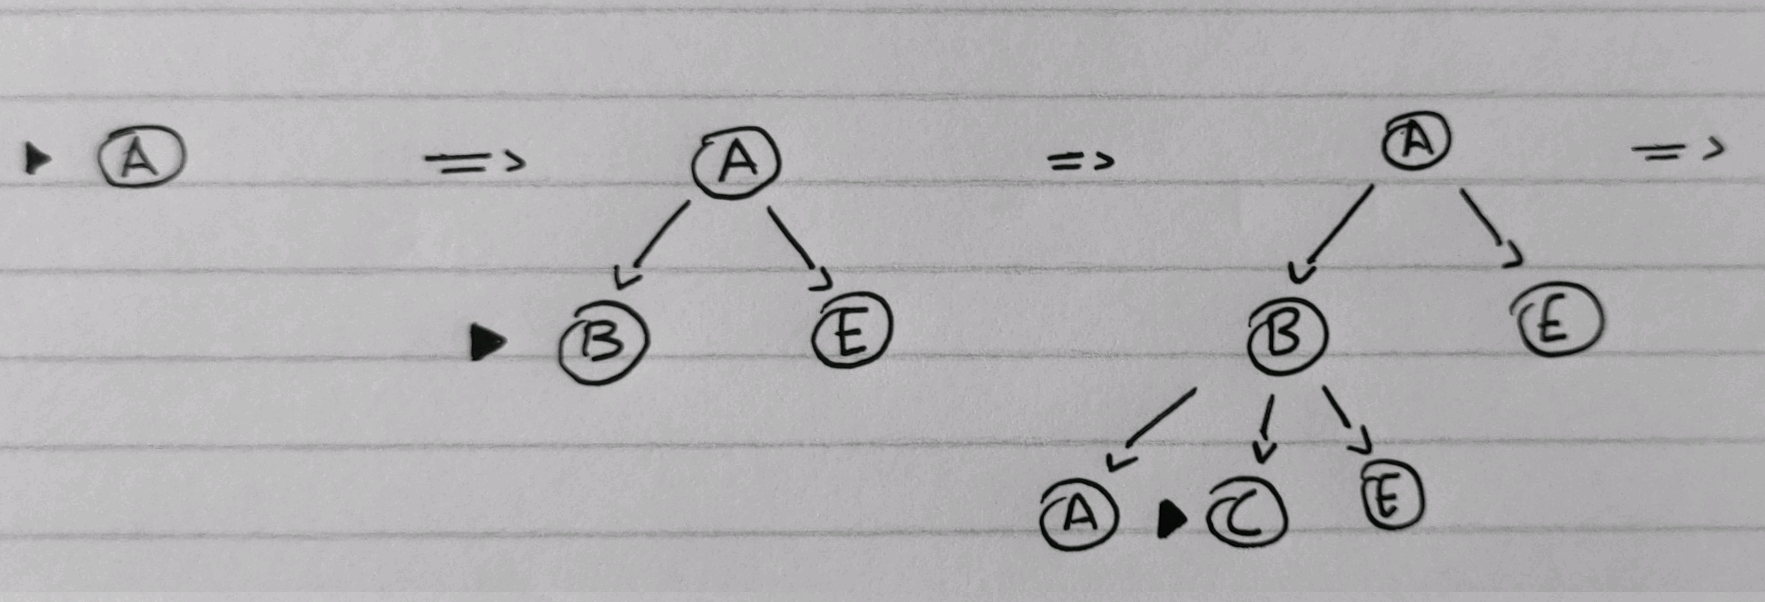
\includegraphics[width=0.45\textwidth]{images/2.jpg}
			\caption{First steps of Depth-First Search. Starting with the initial node A, the deepest node on the frontier is expanded until there are no more successors (deepest point), then returns to the next deepest node on the frontier with unexpanded successors. Depth-First Search is not cost-optimal, as it returns the first solution it finds, even if it is not the cheapest. }
			\label{fig:img2}
		\end{figure}
		
		\begin{figure}[h]
			\centering
			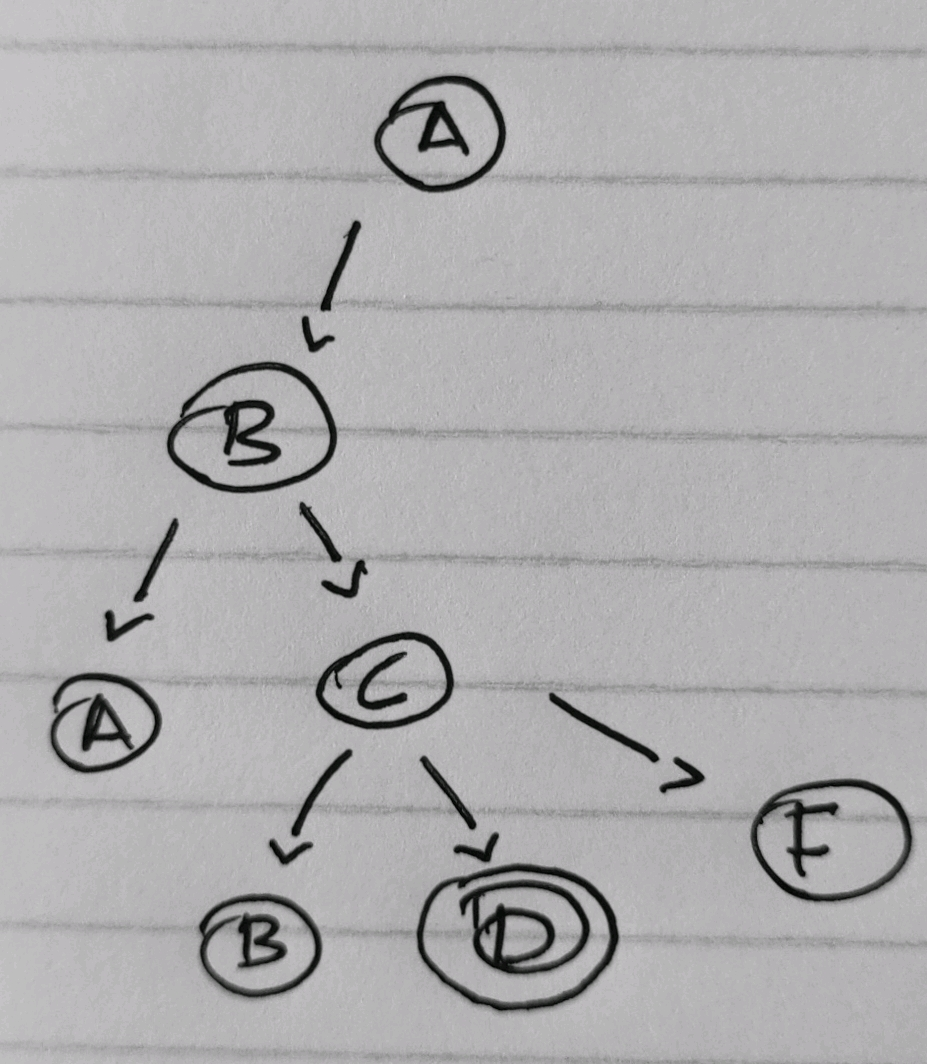
\includegraphics[width=0.25\textwidth]{images/3.jpg}
			\caption{Final step of Depth-First Search, being lucky by reaching the goal state with the optimal path without backtracking and expanding more nodes.}
			\label{fig:img3}
		\end{figure}
	
	    
	    A-star starts by expanding the initial node and proceeds to evaluate each step, a Best-First Search algorithm using the evaluation function $f(n) = g(n) + h(n)$ where $g(n)$ is the path cost from the initial state to node n (the costs for each available transition between states is marked between the edges in \ref{fig:img1}) and $h(n)$ is the estimated cost of the shortest path from $n$ to the goal state. \\
	    
	    Notice that when the goal state $D$ appears on the search tree (\ref{fig:img4}), the A-star algorithm will not settle for a solution with such cost because the unexpanded node $B$ at the frontier indicates that there might be a solution with lower cost through node $B$. That is when, in the next step, node $B$ will be expanded and A-star will lead to the optimal solution. \\
	    
	    As a result we see how in this example, due to the formulation of the problem and the heuristic function $h$, how Depth-First Search was lucky in obtaining the optimal path in fewer steps than A-star, although as we discussed in the first paragraph it is not usually the case. Also A-star is cost-optimal while Depth-First Search is not; it will return the first solution it finds even if not the cheapest.
	     
		\begin{figure}[h]
		\centering
		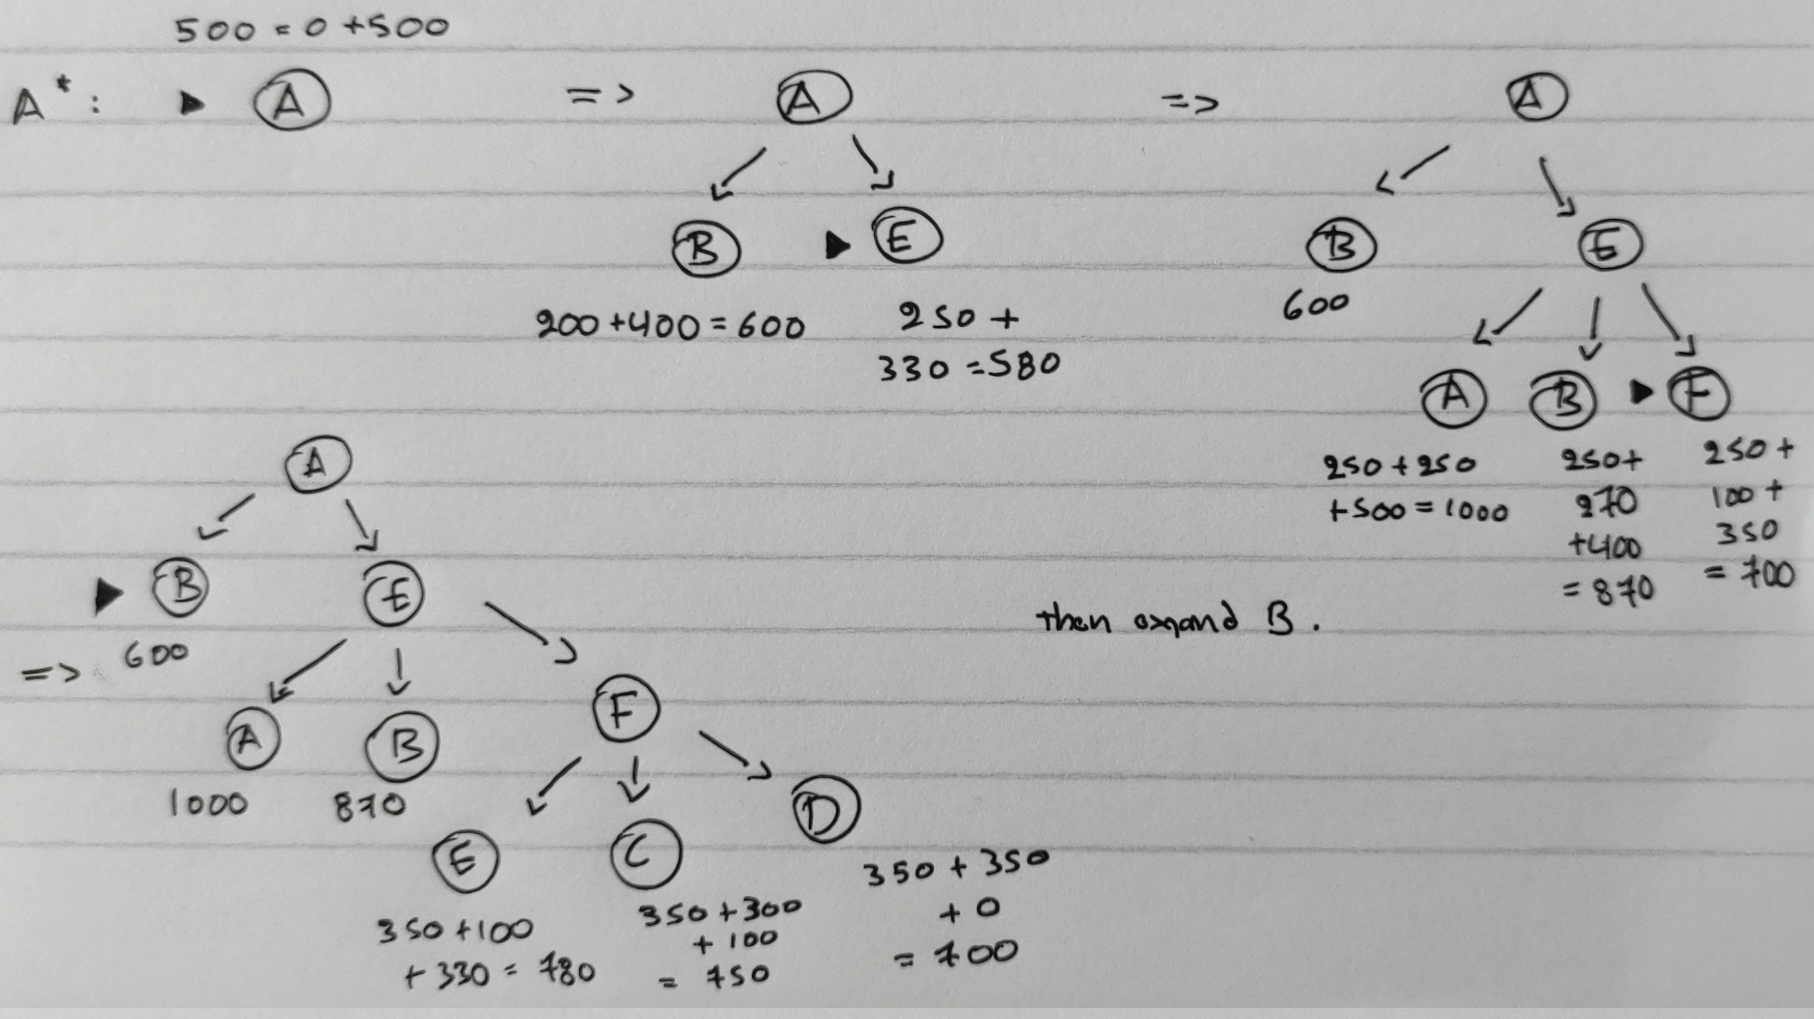
\includegraphics[width=0.85\textwidth]{images/4.jpg}
		\caption{Progress of the $A^\star$ algorithm with the goal of reaching state $D$.}
		\label{fig:img4}
	\end{figure}
			
	\end{Exercise}
	
	\newpage 
	
	\begin{Exercise}[3]
		%Recall that the heuristic function in best-first search is $f(n) = g(n) + h(n)$,
		%where $g(n)$ is the exact cost of getting to the current node $n$, and $h(n)$ is the
		%estimated minimum cost of getting from $n$ to a goal state.
		\begin{enumerate}
			\item Suppose we run a greedy search algorithm with $h(n) = -g(n)$. What sort of
		search will the greedy search emulate?
		
		    \item Sometimes there is no good evaluation function for a problem, but there
		is a good comparison method: a way to tell if one node is better than another,
		without assigning numerical values to either. Show that this is enough to do a
		best-first search. What properties of best-first search do we give up if we only
		have a comparison method? \\
		\end{enumerate}
		
		\solution \\
		
		\begin{enumerate}
			\item The best candidate nodes will be the ones with the longest cost paths, because the deeper the node the better its cost. So it emulates depth-first search (DFS).
			
			\item Best-first search is implemented using a priority queue, so we can still do best-first search by sorting the queue only by comparison between the elements of the queue. But because there is no quantitative information about whether one node is better than an other, we cannot combine the results of the comparison with a function like $g(n)$ or $h(n)$ so we cannot implement $A^{\star}$ search, so we give up completeness and optimality.
		\end{enumerate}
		
	\end{Exercise}
	
	\newpage
	
	\begin{Exercise}[4]
		In this exercise you will run various informed and uninformed search algorithms	to solve the 8-puzzle problem. You can use the code of the book given to you (Note than $\mathrm{Assignment_1.ipynb}$ file need to be inside aima-search folder). The algorithms you can use can be found on search.py. You will have to run the code 100 times for the 8-puzzle, for random puzzles each time. Because some algorithms may take too long to solve a problem, we set an upper limit on the number of states that each algorithm can visit ($10^7$ in our case). In case the	algorithm fails to find a solution (it has reached the limit of the number of states it can visit, it has reached the limit of the memory it can use or for some other reason) the value $-1$ is stored as the number of states and the size of the solution. \\
		
		\textbf{Use at least 4 algorithms of your choice.} \\
		
		You have to compare the algorithms based on the above measurements in terms of the complexity and quality of the solution, since a solution has been found. Also calculate how many times each algorithm found a solution. How you compare them is up to you. For example, you can calculate the transaction factor, various statistics (mean values, standard deviation, etc.), create graphs (see also in the book how search algorithms are compared). You can use whatever tools you want for this purpose and modify the given code accordingly. One should be able to decide which algorithm to use based on your comparison. Also answer the following questions: \\
		
		\begin{itemize}
			\item What results would you expect based on the theory;
			\item Are they verified by experiments? Comment on that.
			\item Which algorithm would you choose to use? Justify your answer.
			\item How does the size of the optimal solution affect the performance of the
			algorithms;
		\end{itemize}
	
		Experiment with the maximum number of states (variable max-actions) (i.e.run the algorithms several times with different variable values). What do you notice? Justify your answers. \\
		
	\end{Exercise}

    \solution \\
    
    For time complexity issues, do the nature of the time complexity of the algorithms, the number of max actions has been set to $10^5$, which still yields meaningful results on the performance of the search algorithms. \\
    
    Used algorithms include A-star Search, Recursive Best-First Search (R-BFS), Depth-First Search (DFS) and Uniform-Cost Search. \\
    
    \begin{lstlisting}[language=Python, caption=Python Code for scatterplot of the running times of Succesful Runs (in seconds) for each Search Algorithm]
    	names = ['A-star', 'Recursive BFS', 'Depth-First Search', 'Uniform-Cost Search']
    	
    	count_values = [count_times, count1_times, count2_times, count3_times]
    	mean_values = [count_mean, count1_mean, count2_mean, count3_mean]
    	var_values = [count_var, count1_var, count2_var, count3_var]
    	
    	plt.figure(figsize=(9, 4))
    	
    	plt.scatter(x=range(1,count+1), y=count_times, label="A-star")
    	plt.scatter(x=range(1,count1+1), y=count1_times, label="Recursive BFS")
    	plt.scatter(x=range(1,count2+1), y=count2_times, label="Depth-First Search")
    	plt.scatter(x=range(1,count3+1), y=count3_times, label="Uniform-Cost Search")
    	plt.suptitle('Running Times of Successful Runs (in seconds)')
    	plt.xlabel("Run")
    	plt.ylabel("seconds")
    	plt.legend()
    	plt.show()
    \end{lstlisting}
		
	We evaluate the performance of the presented algorithms on the basis of completeness, cost optimality, time and space complexity:
	
	\begin{figure}[h]
		\centering
		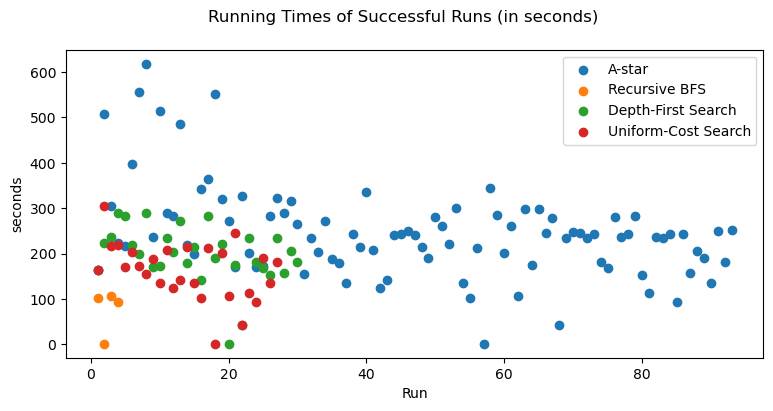
\includegraphics[width=0.75\textwidth]{images/img1.png}
		\caption{Scatterplot of Running Times for each solvable initial state}
	\end{figure}

	\begin{itemize}
		
		\item A-star is complete and optimal, provided $h(n)$ is an admissible heuristic (in our case, in the 8-puzzle problem, it is). The space complexity, which is exponential, is still an issue in practice), which we verify by our experiments.
		
		\item Recursive-BFS is a robust and optimal version of Best-First-Search that uses limited memory resources compared to standard BFS. So given enough time it would solve problems in which A-star runs out of memory.
		
		\item Depth-First Search expands the deepest node first, it is neither complete nor optimal but has linear space complexity.
		
		\item Uniform-Cost Search expands the nodes with the lowest $g(n)$, is optimal for general action costs but running time remains an issue.
	
	\end{itemize}
	 
	 \begin{lstlisting}[caption=Output of the 4 algorithms]
	 	##================##
	 	Total random initial states: 100
	 	That are solvable: 100
	 	A-star: 93 successes
	 	Recursive BFS: 4 successes
	 	Depth-First Search: 30 successes
	 	Uniform-Cost Search:  27 successes
	 	##================##
	 	A-star mean time: 246.57977447714856
	 	Recursive BFS mean time: 75.70691114664078
	 	Depth-First Mean time: 197.30689787069957
	 	Uniform-Cost Search Mean time: 162.12999637921652
	 	##================##
	 	A-star variance time: 10686.768832753627
	 	Recursive BFS variance time: 2482.7021897812915
	 	Depth-First variance time: 4076.8551931757356
	 	Uniform-Cost variance time: 3998.614603300636
	 	--- Elapsed Time: 26375.817984342575 seconds ---
	 \end{lstlisting}
	\begin{figure}[h]
		\centering
		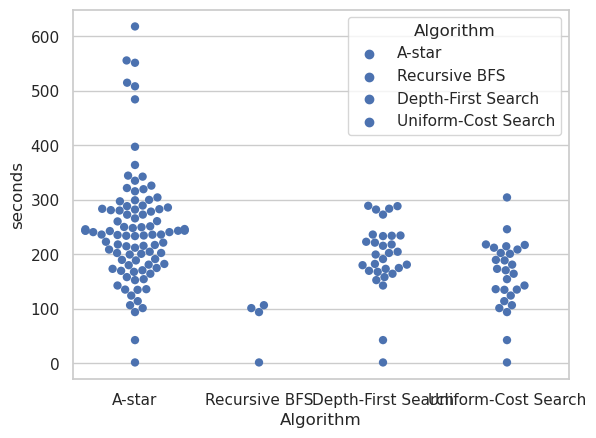
\includegraphics[width=0.55\textwidth]{images/img2.png}
		\caption{Swarmplot of the Running Times of Successful Runs (in seconds)}
	\end{figure}

    \begin{figure}[h]
    	\centering
    	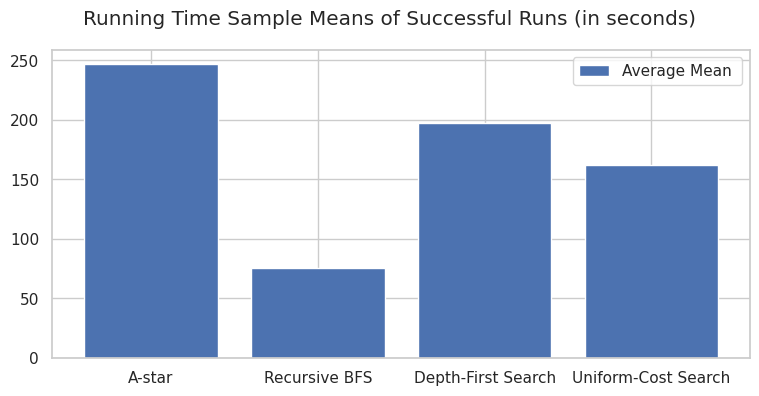
\includegraphics[width=0.55\textwidth]{images/img3.png}
    	\caption{Running Time Sample Means of Successful Runs (in seconds)}
    \end{figure}

    \begin{figure}[h]
    	\centering
    	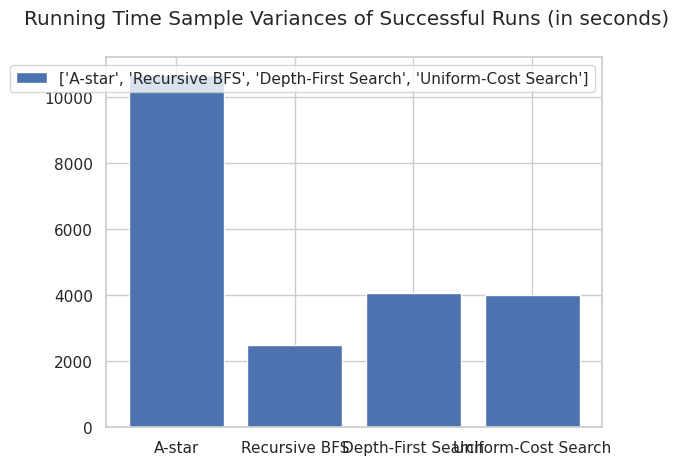
\includegraphics[width=0.55\textwidth]{images/img4.png}
    	\caption{Running Time Sample Variances of Successful Runs (in seconds)}
    \end{figure}

We begin by testing 100 solvable initial random states, with an upper bound for the total number of actions. We then generate a scatterplot with the running times of the succesful runs (the ones that reach a goal state) as well as a barplot with the mean and variance of each algorithm. A swarmplot (similar to a boxplot) is also generated, to give a broader picture of each sample distribution and outliers. \\

With the number of maximum actions we have specified, A-star has reached the goal state in almost every of the solvable initial states, in general using more running time but with much higher variance in the sample runs. RBFS has reached only a handful of them, while Depth-First and Uniform-Cost search have performed in a very similar manner. \\

To assert whether the four algorithms perform different that each other, we conduct pairwise t-tests, on a significance level $\alpha = 0.05$, a total of $4\choose2$ = 6 times assuming False variances in all cases except with Depth-First Search and Uniform-Cost Search where our sample variances appear highly similar in value. The Hypothesis testing between the true means $\mu_0$ and $\mu_1$ of the two paired samples is: $$H_0: ~\mu_0 = \mu_1, ~H_1: ~\mu_0 \neq \mu_1$$

\begin{lstlisting}[language=Python, caption=Example of Paired t-test between Depth-First Search and Uniform-Cost Search assuming equal variance in the distribution]
print("Pairwise t-test for running times of Depth-First Search and Uniform-Cost Search:", 
stats.ttest_ind(a=count2_times, b=count3_times, equal_var=True))

\end{lstlisting}

Our significance level $a$ corresponds to  Error type I which is the Probability we reject the null hypothesis if true. A p-value less than a indicates strong evidence against the null hypothesis, hence the null hypothesis not accepted. A p-value higher than a indicates strong evidence supporting the null hypothesis, hence the null hypothesis is accepted. \\

For each test, we get a p-value of $0.0027$, $0.0025$, $1.8315$, $0.009$, $0.0297$ and $0.04160$ respectively. Hence A-star on average performs slower than DFS and Uniform-Cost Search, while for Recursive BFS our data does not give us a clear distinction between the running times of the two algorithms from our 100 solvable initial states. \\

Due to the informed nature of A-star, as well as the fact that it is complete and optimal, it would generally be our first choice for a Search Algorithm in practice. By expanding the allowed number of actions, A-star finds a solution to all 100 solvable initial states, while other algorithms waste enormous amounts of running time and failing to reach a goal state due to not being complete. By lowering the amount of maximum actions, most fail to reach the goal state, as expected, unless they get "lucky" with the initial state, requiring a few number of actions. Even in these cases, A-star finds most solutions rather quickly. \\

Full Code listing is available at the accompanied .ipynb Jupyter Notebook, as well as at the appendix of this document.

\newpage

\appendix

\begin{lstlisting}[language=Python, caption=Full Code Listing]
    from search import * #import all search algorithms
	import time  
	import random
	import timeit
	
	import matplotlib.pyplot as plt #use matplotlib for easthetic plots 
	import seaborn as sns #for swarmplot
	import numpy as np
	import pandas as pd
	
	import statistics #for mean and variance
	import scipy.stats as stats #for hypothesis testing
	
	class EightPuzzle(Problem):
	      """ The problem of sliding tiles numbered from 1 to 8 on a 3x3 board, where one of the
	      squares is a blank. A state is represented as a tuple of length 9, where  element at
	      index i represents the tile number  at index i (0 if it's an empty square) """
	
	      max_actions = 10**5 #limit for number of actions
	      current_actions = 0
	
	      def __init__(self, initial, goal=(1, 2, 3, 4, 5, 6, 7, 8, 0)):
	          """ Define goal state and initialize a problem """
	          super().__init__(initial, goal)
		
	      def find_blank_square(self, state):
	          """Return the index of the blank square in a given state"""
	
	          return state.index(0)
	
	      def actions(self, state):
	          """ Return the actions that can be executed in the given state.
	          The result would be a list, since there are only four possible actions
	          in any given state of the environment """
	
	          possible_actions = ['UP', 'DOWN', 'LEFT', 'RIGHT']
	          index_blank_square = self.find_blank_square(state)
	
	          if index_blank_square % 3 == 0:
	          possible_actions.remove('LEFT')
	          if index_blank_square < 3:
	             possible_actions.remove('UP')
	          if index_blank_square % 3 == 2:
	             possible_actions.remove('RIGHT')
	          if index_blank_square > 5:
	             possible_actions.remove('DOWN')
	
	          return possible_actions
	
	      def result(self, state, action):
	          """ Given state and action, return a new state that is the result of the action.
	          Action is assumed to be a valid action in the state """
	
           	  # blank is the index of the blank square
	          blank = self.find_blank_square(state)
	          new_state = list(state)
	
           	  delta = {'UP': -3, 'DOWN': 3, 'LEFT': -1, 'RIGHT': 1}
	          neighbor = blank + delta[action]
	          new_state[blank], new_state[neighbor] = new_state[neighbor], new_state[blank]
	          self.current_actions +=1
	          return tuple(new_state)
	
	      def goal_test(self, state):
	          """ Given a state, return True if state is a goal state or False, otherwise """
	
	          return (state == self.goal) or (self.current_actions>self.max_actions)
	
   	      def check_solvability(self, state):
	          """ Checks if the given state is solvable """
	
	          inversion = 0
	          for i in range(len(state)):
	              for j in range(i + 1, len(state)):
	                  if (state[i] > state[j]) and state[i] != 0 and state[j] != 0:
	                      inversion += 1
	
	          return inversion % 2 == 0
	
     	  def h(self, node):
	          """ Return the heuristic value for a given state. Default heuristic function used is 
	          h(n) = number of misplaced tiles """
	
	          return sum(s != g for (s, g) in zip(node.state, self.goal))
	
    def run_singleTest(initial_state):
	
        puzzle = EightPuzzle(initial_state)
	    results = []        
	
	    puzzle.current_actions = 0 
	          
	    # start timing your execution
	    t0 = time.time()
	          
	    # save important parameters
	    algorithm_results = {'Algorithm': 'A-star', #informed search
		              'Initial State': initial_state,
		              'Final_State': astar_search(puzzle)} 
	
	    t1 = time.time() - t0
	    algorithm_results['Time'] = t1
	    results.append(algorithm_results)
	
	    ############
	    puzzle.current_actions = 0 
	    # start timing your execution
	    t0 = time.time()
	    # save important parameters
	    algorithm_results = {'Algorithm': 'RBFS', #uninformed
		              'Initial State': initial_state, #u
		              'Final_State': recursive_best_first_search(puzzle)} 
	
	    t1 = time.time() - t0
	    algorithm_results['Time'] = t1
	    results.append(algorithm_results)
	
	    ############
	    puzzle.current_actions = 0 
	    # start timing your execution
	    t0 = time.time()
	    # save important parameters
	    algorithm_results = {'Algorithm': 'Depth-First Search', #uninformed
		              'Initial State': initial_state,
		              'Final_State': depth_first_graph_search(puzzle)} #breadth_first_search very slow to converge
	
	    t1 = time.time() - t0
	    algorithm_results['Time'] = t1
	    results.append(algorithm_results)
	
	    #############  
	    puzzle.current_actions = 0 
	    # start timing your execution
	    t0 = time.time()
	    # save important parameters
	    algorithm_results = {'Algorithm': 'Uniform-Cost Search', #very slow to converge
		              'Initial State': initial_state, 
		              'Final_State':  uniform_cost_search(puzzle)} 
	    t1 = time.time() - t0
	    algorithm_results['Time'] = t1
	    results.append(algorithm_results)
	
	    return results
	
	t0 = time.time()
	
	goal = (1, 2, 3, 4, 5, 6, 7, 8, 0)
	print('Goal:', goal)
	
	size = 10**2 #total number of initial states
	
	count = count1 = count2 = count3 = 0
	total_solvables = 0
	
	#running times for each initial solution (in seconds)
	count_times = []
	count1_times = []
	count2_times = []
	count3_times = []
	
	i=0
	
	#while (i < size+1): #test any initial state 
	while(total_solvables < 100): #test solvable initial states only
	    initial_state = tuple(random.sample(list(goal),9))
	
	    #check if chosen initial state is solvable 
	    solvable = EightPuzzle(initial_state).check_solvability(initial_state)
	
	    if(not solvable):
	        print('Initial State unsolvable, moving to the next one:')
	    else:
	        total_solvables +=1;       
	        t_solve0 = time.time()
	
	        results = run_singleTest(initial_state)
	        print('Initial State', i , ':', str(initial_state))
	
	        for result in results:
	            if result['Final_State'].state == goal:
	                if(str(result['Algorithm']) == 'A-star'):
	                    count+=1
	                    count_times.append(time.time() - t_solve0)
	                elif(str(result['Algorithm']) == 'RBFS'):
	                    count1+=1
	                    count1_times.append(time.time() - t_solve0)
	                elif(str(result['Algorithm']) == 'Depth-First Search'):
	                    count2+=1
	                    count2_times.append(time.time() - t_solve0)
	                elif(str(result['Algorithm']) == 'Uniform-Cost Search'):
	                    count3+=1
	                    count3_times.append(time.time() - t_solve0)
	
                 	print('Algorithm: ' + str(result['Algorithm']) + ' succeeded , Execution Time: ' + str(round(result['Time'],2)), 's')
	                print('Resulting solution: ' + str(result['Final_State'].solution()) + ' ending in board: ' + str(result['Final_State'].state))
	                print('-=-=-=-=-=-=-=-=-')
	            else:
	                print('Algorithm: ' + str(result['Algorithm']) + ' failed , Execution Time: ' + str(round(result['Time'],2)),'s')
	                print('Resulting solution: ' + str(result['Final_State'].solution()) + ' ending in board: ' + str(result['Final_State'].state))
	                print('-=-=-=-=-=-=-=-=-')
	i=i+1
	
	count_mean = count1_mean = count2_mean = count3_mean = 0
	
	count_var = count1_var = count2_var = count3_var = 0
	
	if(len(count_times) > 0):
	    count_mean = statistics.mean(count_times)
	    count_var = statistics.variance(count_times)
	
	if(len(count1_times) > 0):
	    count1_mean = statistics.mean(count1_times)
	    count1_var = statistics.variance(count1_times)
	
	if(len(count2_times) > 0):
	    count2_mean = statistics.mean(count2_times)
	    count2_var = statistics.variance(count2_times)
	
	if(len(count3_times) > 0):
	    count3_mean = statistics.mean(count3_times)
	    count3_var = statistics.variance(count3_times)
	
	print('##================##')
	#print('Max Actions:', max_actions)
	print('Total random initial states:', size)
	print('That are solvable:', total_solvables)
	print('A-star:', count, 'successes')
	print('Recursive BFS:', count1, 'successes')
	print('Depth-First Search:', count2, 'successes')
	print('Uniform-Cost Search: ', count3, 'successes')
	print('##================##')
	print('A-star mean time:', count_mean)
	print('Recursive BFS mean time:', count1_mean)
	print('Depth-First Mean time:', count2_mean)
	print('Uniform-Cost Search Mean time:', count3_mean)
	print('##================##')
	print('A-star variance time:', count_var)
	print('Recursive BFS variance time:', count1_var)
	print('Depth-First variance time:', count2_var)
	print('Uniform-Cost variance time:', count3_var)
	print("--- Elapsed Time: %s seconds ---" % (time.time() - t0))
	
	names = ['A-star', 'Recursive BFS', 'Depth-First Search', 'Uniform-Cost Search']
	
	count_values = [count_times, count1_times, count2_times, count3_times]
	mean_values = [count_mean, count1_mean, count2_mean, count3_mean]
	var_values = [count_var, count1_var, count2_var, count3_var]
	
	plt.figure(figsize=(9, 4))
	
	plt.scatter(x=range(1,count+1), y=count_times, label="A-star")
	plt.scatter(x=range(1,count1+1), y=count1_times, label="Recursive BFS")
	plt.scatter(x=range(1,count2+1), y=count2_times, label="Depth-First Search")
	plt.scatter(x=range(1,count3+1), y=count3_times, label="Uniform-Cost Search")
	plt.suptitle('Running Times of Successful Runs (in seconds)')
	plt.xlabel("Run")
	plt.ylabel("seconds")
	plt.legend()
	plt.show()
		
	sns.set(style="whitegrid")	
	sns.swarmplot(x="Algorithm", y="seconds", data=pd.DataFrame({"seconds": count_values[0],"Algorithm": names[0]}), size=6, hue='Algorithm')
	sns.swarmplot(x="Algorithm", y="seconds", data=pd.DataFrame({"seconds": count_values[1],"Algorithm": names[1]}), size=6, hue='Algorithm')
	sns.swarmplot(x="Algorithm", y="seconds", data=pd.DataFrame({"seconds": count_values[2],"Algorithm": names[2]}), size=6, hue='Algorithm')
	sns.swarmplot(x="Algorithm", y="seconds", data=pd.DataFrame({"seconds": count_values[3],"Algorithm": names[3]}), size=6, hue='Algorithm')
	plt.show()
		
	plt.figure(figsize=(9, 4))
	
	plt.bar(names, mean_values, label="Average Mean ")
	plt.suptitle('Running Time Sample Means of Successful Runs (in seconds)')
	plt.legend()
	plt.show()
	
	plt.bar(names, var_values, label= names)
	plt.suptitle('Running Time Sample Variances of Successful Runs (in seconds)')
	plt.legend()
	
	print("Pairwise t-test for running times of A-star and  RBFS",
	stats.ttest_ind(a=count_times, b=count1_times, equal_var=False))
	
	print("Pairwise t-test for running times of A-star and Depth-First Search:",
	stats.ttest_ind(a=count_times, b=count2_times, equal_var=False))
	
	print("Pairwise t-test for running times of A-star and Uniform-Cost Search:", 
	stats.ttest_ind(a=count_times, b=count3_times, equal_var=False))
	
	print("Pairwise t-test for running times of RBFS and Depth-First Search:", 
	stats.ttest_ind(a=count1_times, b=count2_times, equal_var=False))
	
	print("Pairwise t-test for running times of RBFS and Uniform-Cost Search:", 
	stats.ttest_ind(a=count1_times, b=count3_times, equal_var=False))
	
	print("Pairwise t-test for running times of Depth-First Search and Uniform-Cost Search:", 
	stats.ttest_ind(a=count2_times, b=count3_times, equal_var=True))
	
\end{lstlisting}

\end{document}
